\pagebreak
\subsection{Task 1 - Building a VMware Environment}
For this demonstration secure data centre environment setup, I installed ESXi inside VMware Workstation 12 on my University of South Wales Applied Cyber Security designated workstation. This allowed me to use a single physical machine to manage and screenshot (via VMware's `Print Screen' functionality) the ESXi installation directly, manage the servers installed inside ESXi via the vSphere Web Client and vSphere Client (desktop), and test the configuration from a Windows 10 Enterprise client that was also installed inside VMware Workstation 12.

In a real-world deployment of ESXi, it would be installed bare-metal -- in other words, ESXi would be installed directly onto the physical hardware as the primary Operating System and would then be managed remotely for the most part.

\bigskip
\noindent The process for building the VMware environment is as follows:

\subsubsection*{Download the vSphere environment software}
\begin{enumerate}[series=task1methodology]
  \item Download the vSphere environment from the \textit{OnTheHub\textsuperscript{\textregistered}} website\footnote{\url{https://onthehub.com/}}.
\end{enumerate}

\noindent From Figure~\ref{fig:task1:01_downloadvsphere} in the \nameref{app:ancillaryscreenshots} appendix, it shows that three pieces of software are available for download. It should be noted here that it is not made explicitly clear that the `VMware-VMvisor-Installer-6.0.0.update02-3620759.x86\_64.iso` is an installer for an updated version of ESXi 6.0.0 and is not an updated version of ESXi 6.5. As a result of this confusion, I initially installed the wrong version of ESXi insider VMware Workstation. In the methodology, I will include instructions for updating ESXi from version 6.0 to 6.5.

\subsubsection*{Create a new virtual machine in VMware Workstation}
\begin{enumerate}[resume*=task1methodology]
  \item Create a new virtual machine for ESXi in VMware Workstation 12. I have highlighted some notable steps below:
    \begin{enumerate}[label=(\alph*)]
      \item Select the ESXi ISO in the `Guest Operating System Installation' step.
        % \begin{minipage}{\linewidth}
        \begin{figure}[H]
          \centering
          \captionsetup{skip=2pt}
          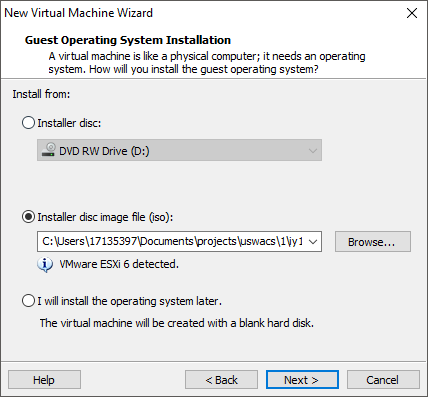
\includegraphics{task1_02_vmwareinstall_02}
          \caption{Selecting the ESXi ISO for installation into the new VM}
          \label{fig:task1:02_vmwarewiz_02}
        \end{figure}
        % \end{minipage}
      \item Increase the `Number of processors' and `Number of cores per processor' in the `Processor Configuration' step as several VMs will be running within this ESXi VM.
        \begin{figure}[H]
          \centering
          \captionsetup{skip=2pt}
          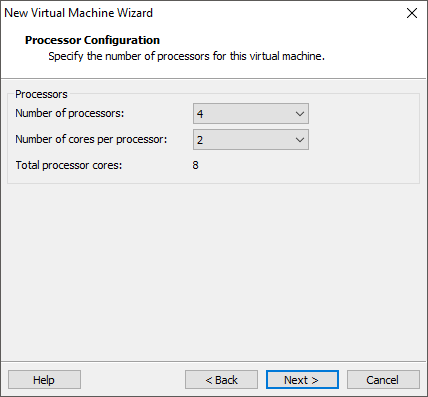
\includegraphics{task1_02_vmwareinstall_03}
          \caption{Increasing the number of processors for the ESXi VM}
          \label{fig:task1:02_vmwarewiz_03}
        \end{figure}
      \item Increase the amount of memory allocated to the ESXi VM in the `Memory for the Virtual Machine' step as several VMs will be running within this ESXi VM. With consideration of the failover configuration of Task 2 \todo{ref this}, I decided to give the VM 16GB of memory. This would allow each of the 4 VMs inside ESXi \textit{(2 servers and a failover for each)} to have 4GB of memory.
        \begin{figure}[H]
          \centering
          \captionsetup{skip=2pt}
          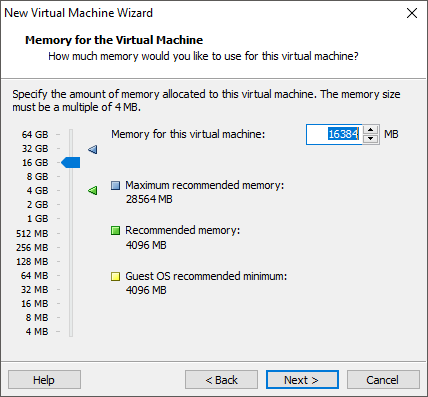
\includegraphics{task1_02_vmwareinstall_04}
          \caption{Increasing the amount of memory for the ESXi VM}
          \label{fig:task1:02_vmwarewiz_04}
        \end{figure}
      \item Setup the `Host-only Network' only in the `Network Type' step. I will add the `NAT Adapter' later and demonstrate how to configure ESXi to use it correctly at that time.
        \begin{figure}[H]
          \centering
          \captionsetup{skip=2pt}
          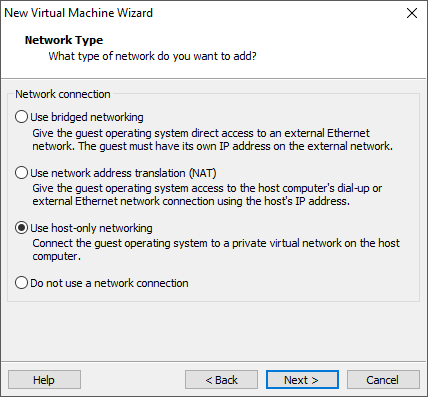
\includegraphics{task1_02_vmwareinstall_05}
          \caption{Configuring the initial network adapter for the VM}
          \label{fig:task1:02_vmwarewiz_05}
        \end{figure}
      \item Increase the maximum disk size in the `Specify Disk Capacity' step to 200GB. This will allow each of the VMs inside ESXi to have 40GB of space for 4x40=160GB of VMs and then 40GB extra for ESXi to use for storing the server install ISO, snapshots, et cetera.
        \begin{figure}[H]
          \centering
          \captionsetup{skip=2pt}
          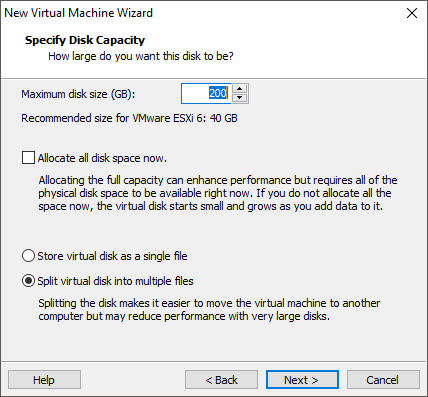
\includegraphics{task1_02_vmwareinstall_08}
          \caption{Setting the maximum disk size for the VM}
          \label{fig:task1:02_vmwarewiz_08}
        \end{figure}
    \end{enumerate}
\end{enumerate}

\subsubsection*{Install ESXi in the new virtual machine}
\begin{enumerate}[resume*=task1methodology]
  \item Start the new ESXi VM in VMware Workstation.
\end{enumerate}

\noindent Upon attempting to start the ESXi VM I received the pop-up window shown in Figure~\ref{fig:task1:02_vmwarewiz_11_issue}.

\begin{figure}[H]
  \centering
  \captionsetup{skip=2pt}
  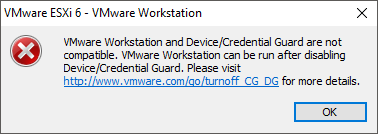
\includegraphics{task1_02_vmwareinstall_11_issue1}
  \caption{VMware issue with Device/Credential Guard}
  \label{fig:task1:02_vmwarewiz_11_issue}
\end{figure}

\noindent Following the link provided in the pop-up redirected me to `VMware Knowledge Base Article 2146361'\footnote{\url{https://kb.vmware.com/s/article/2146361}}. Following steps 1 and 2, as detailed on the site under `Resolution' fixed the issue. I have included screenshots of these steps as Figures~\ref{fig:task1:02_vmware_11_res1} and~\ref{fig:task1:02_vmware_11_res2} in the \nameref{app:ancillaryscreenshots} appendix. After completing this resolution process, I was able to start the ESXi VM in VMware Workstation successfully and continued with the task.

\begin{enumerate}[resume*=task1methodology]
  \item Step through the EXSi installer. I have highlighted some notable steps below:
    \begin{enumerate}[label=(\alph*)]
      \item Select the local storage device.
        \begin{figure}[H]
          \centering
          \captionsetup{skip=2pt}
          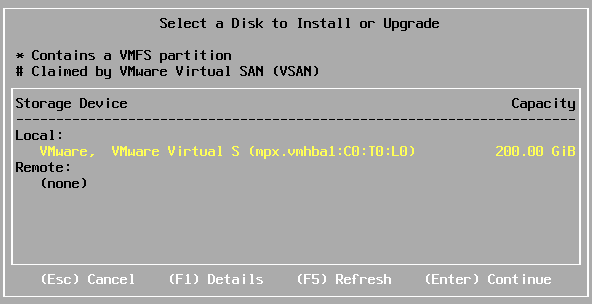
\includegraphics[width=\textwidth]{VMware_ESXi_6-2018-05-08-17-41-37_crop}
          \caption{Selecting the local storage device in the ESXi install}
          \label{fig:task1:esxiinstall_01}
        \end{figure}
      \item Select `United Kingdom' as the keyboard layout.
        \begin{figure}[H]
          \centering
          \captionsetup{skip=2pt}
          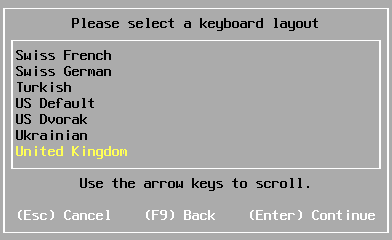
\includegraphics{VMware_ESXi_6-2018-05-08-17-41-48_crop}
          \caption{Selecting the keyboard layout in the ESXi install}
          \label{fig:task1:esxiinstall_02}
        \end{figure}
      \item Setting the `root' password -- in a real-world installation it should be unique, relatively long; and contain a wide combination of letters (both lowercase and uppercase), numbers, and symbols. This password will be used to login via the vSphere Web or Desktop Clients in order to manage the ESXi remotely. It is also used as the password for logging into the ESXi via SSH.
        \begin{figure}[H]
          \centering
          \captionsetup{skip=2pt}
          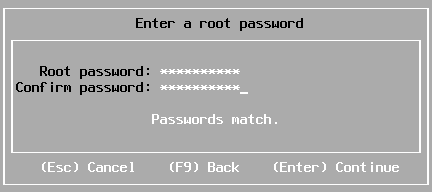
\includegraphics{VMware_ESXi_6-2018-05-08-17-42-30_crop}
          \caption{Setting the root password in the ESXi install}
          \label{fig:task1:esxiinstall_03}
        \end{figure}
      \item Confirm the installation of ESXi.
        \begin{figure}[H]
          \centering
          \captionsetup{skip=2pt}
          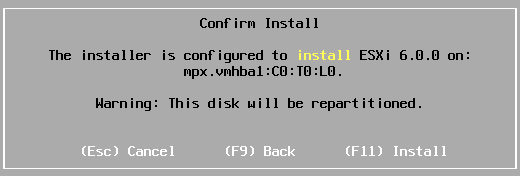
\includegraphics[width=\textwidth]{VMware_ESXi_6-2018-05-08-17-44-17_crop}
          \caption{Confirm the ESXi installation}
          \label{fig:task1:esxiinstall_04}
        \end{figure}
      \item Reboot to complete the ESXi installation.
        % \begin{figure}[H]
        %   \centering
        %   \captionsetup{skip=2pt}
        %   
\includegraphics{VMware_ESXi_6-2018-05-08-17-47-59_crop}
        %   \caption{Reboot in order to complete the ESXi installtion}
        %   \label{fig:task1:esxiinstall_04}
        % \end{figure}
      \item After the ESXi instance has rebooted, make a note of the IPv4 and IPv6 addresses of the instance. In my case these were:
      \begin{itemize}[leftmargin=1.5cm]
        \item [IPv4:] \texttt{192.168.254.136}
        \item [IPv6:] \texttt{[fe80::20c:29ff:fe6b:7530]}
      \end{itemize}
      These can be seen in the screenshot in Figure~\ref{fig:task1:esxiinstall_up} in the \nameref{app:ancillaryscreenshots} appendix.
    \end{enumerate}
\end{enumerate}

\noindent It should be noted that the IPv6 address is marked as `STATIC' rather than `DHCP' -- I have decided to use this address to connect to the ESXi instance as this will prevent issues related to the IPv4 address possibly changing in the event I restart the ESXi VM, restart VMware Workstation, or restart my physical workstation.

\subsubsection*{Connecting to the ESXi instance}
Several methods exist for managing the ESXi instance remotely -- primarily they are the vSphere Client (desktop) and vSphere Web Client. I will detail how to use both below.

\begin{enumerate}[resume*=task1methodology]
  \item Connect to the ESXi instance:
    \begin{enumerate}[label=(\alph*)]
      \item via the vSphere Client (desktop):
        \begin{enumerate}[label=\roman*.]
          \item Install the vSphere Client (desktop) from the\\`VMware-viclient-all-6.0.0-3562874.exe' that was downloaded as part of the vSphere environment package from \textit{OnTheHub\textsuperscript{\textregistered}}.
            \begin{figure}[H]
              \centering
              \captionsetup{skip=2pt}
              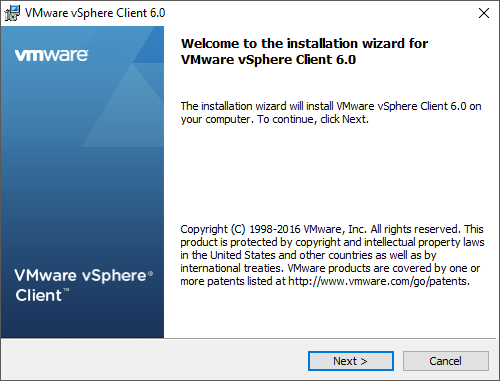
\includegraphics{task1_04_vsphereclientinstall_1}
              \caption{Running the vSphere Client (desktop) installer}
              \label{fig:task1:vspheredesktopclient_01}
            \end{figure}
          \item Start `VMware vSphere Client'.
            \begin{figure}[H]
              \centering
              \captionsetup{skip=2pt}
              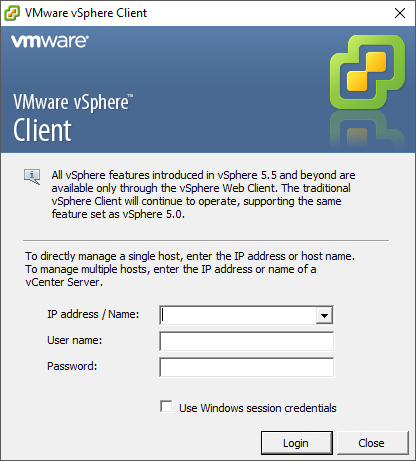
\includegraphics{task1_04_vsphereclientinstall_4}
              \caption{Running the vSphere Client (desktop)}
              \label{fig:task1:vspheredesktopclient_02}
            \end{figure}
          \item Connect to the EXSi instance using the IPv6 address. At the first connection, a pop-up warning about the certificate appears. Before ignoring this, I checked the thumbprint of the certificate against the `SSL Thumbprint (SHA1)' reported in the ESXi instance. This is shown in Figure~\ref{fig:task1:vspheredesktopclient_03} in the \nameref{app:ancillaryscreenshots} appendix.
            \begin{figure}[H]
              \centering
              \captionsetup{skip=2pt}
              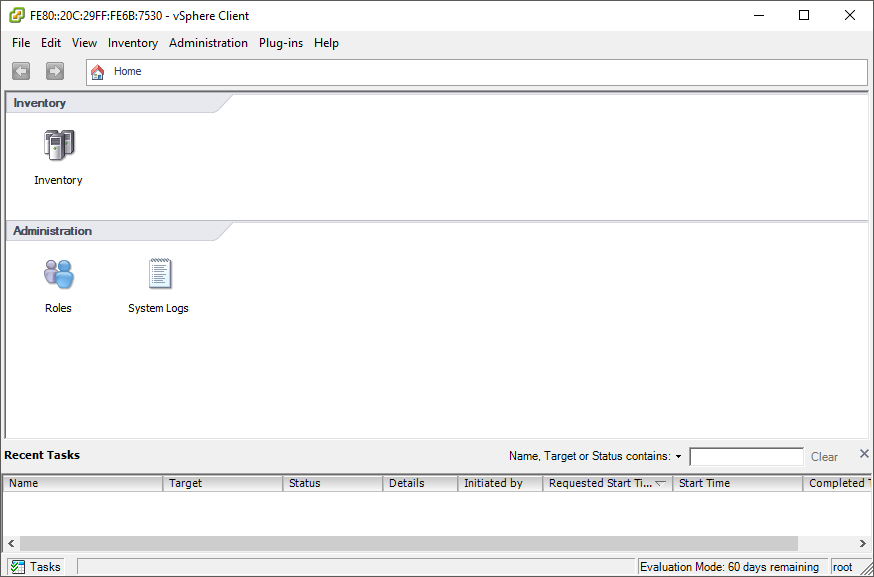
\includegraphics[width=\textwidth]{task1_04_vsphereclientinstall_6}
              \caption{Connected to the ESXi instance using the vSphere Client and IPv6}
              \label{fig:task1:vspheredesktopclient_04}
            \end{figure}
        \end{enumerate}
      \item via the vSphere Web Client:
        \begin{enumerate}[label=\roman*.]
          \item Connect to \texttt{\url{https://[fe80::20c:29ff:fe6b:7530]/ui/}}. Figures~\ref{fig:task1:esxiwebui_01} and~\ref{fig:task1:esxiwebui_02} in the \nameref{app:ancillaryscreenshots} appendix show the login and host overview pages of the Web Client respectively.
        \end{enumerate}
    \end{enumerate}
\end{enumerate}

\noindent On the vSphere Client (desktop) `Connection' window (as shown in Figure~\ref{fig:task1:vspheredesktopclient_02}), it says ``All vSphere features introduced in vSphere 5.5. and beyond are available only through the vSphere Web Client. The traditional vSphere Client will continue to operate, supporting the same feature set as vSphere 5.0.'' Due to this, I decided to, as far as possible, manage the ESXi instance via the Web Client interface. I did, however, have to use the vSphere Client (desktop) for some tasks such as configuring the instance to use the NAT adapter correctly.
